\documentclass[11pt, a5paper, parskip=half-, DIV=12]{scrartcl}

\usepackage{../endeavour}
\usepackage{../endeavour_book}

\version{0.2}

\begin{document}
% Colour Cover
\thispagestyle{plain}
\AddToShipoutPictureBG{
\begin{tikzpicture}[remember picture, overlay]
	\node () at (current page.center) {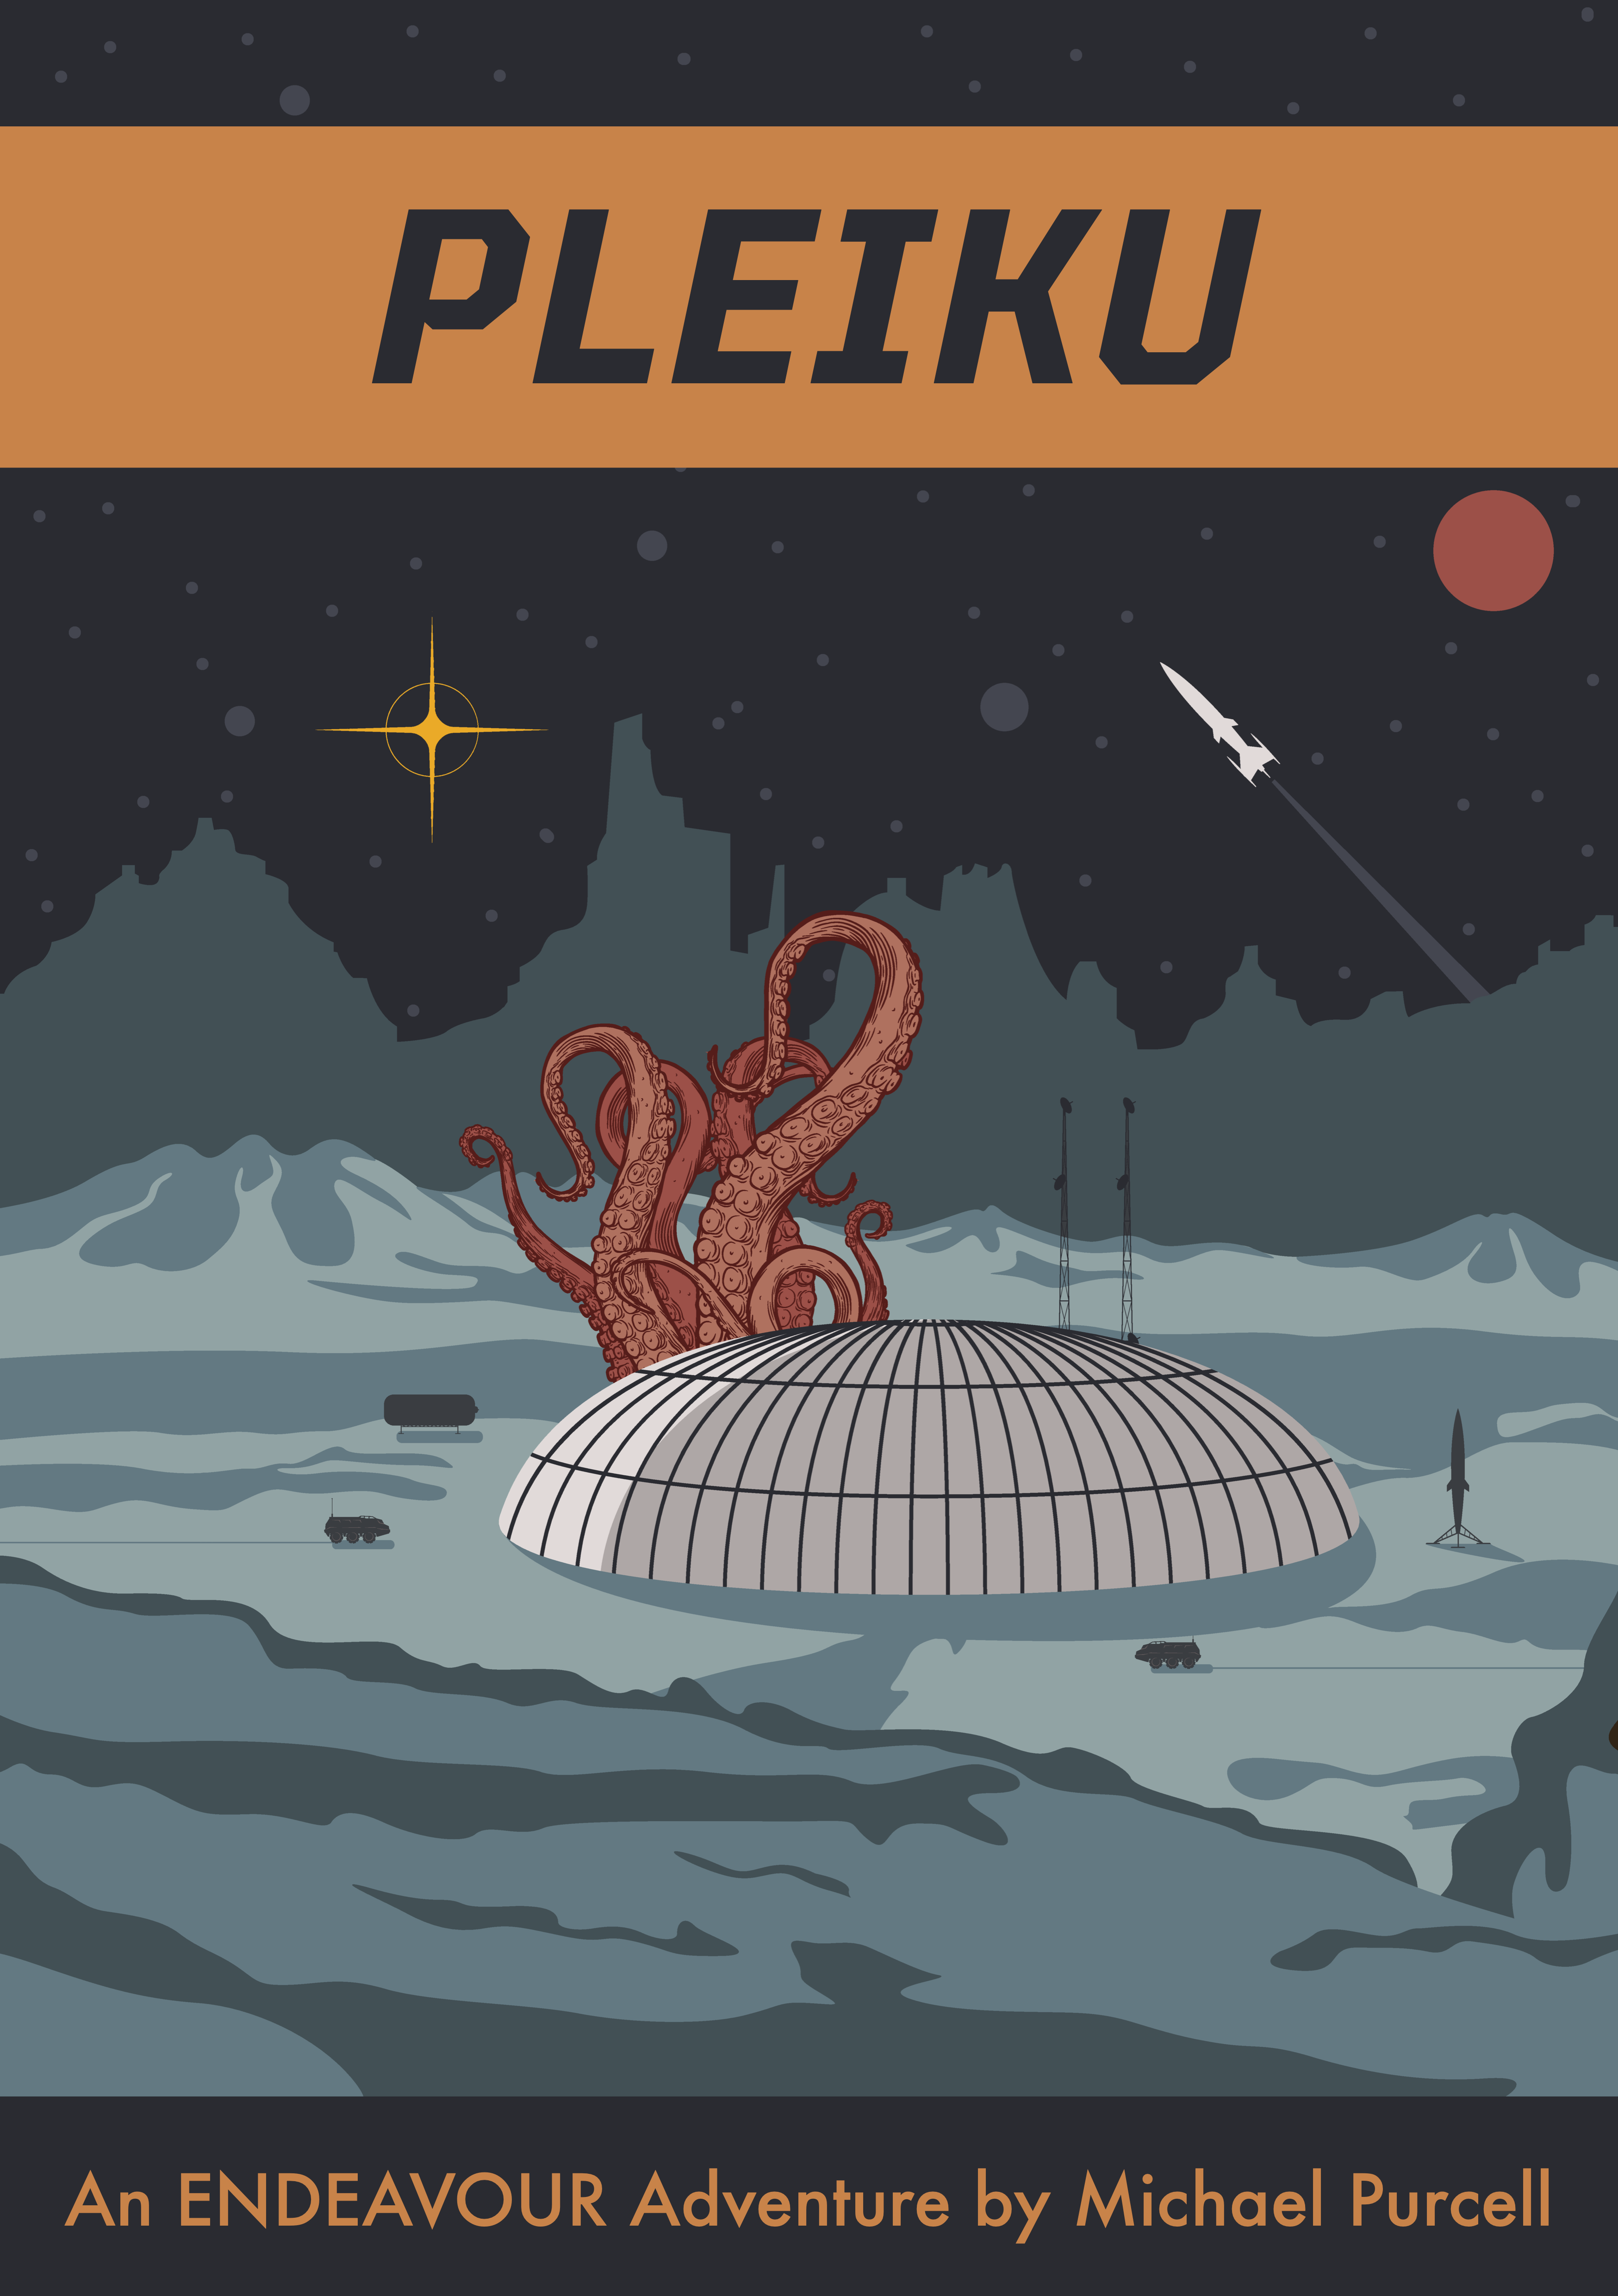
\includegraphics[width=\pagewidth, height=\pageheight]{../Images/pleiku_cover.png}};
\end{tikzpicture}
}
{
\colorlet{headfootcolor}{LCARS_ORANGE}
\phantom{a}

\newpage
}

\ClearShipoutPicture
\AddToShipoutPictureBG{
	\begin{tikzpicture}[remember picture, overlay]
	\pic () at (current page.center) {starfield};
		\node[endeavour_box, minimum width=12.6cm, minimum height=18.8 cm] at (current page.center) {};
	\end{tikzpicture}
}

\setcounter{page}{1}
\setmainfont{TeX Gyre Schola}
\normalsize
\raggedright

\section*{Pleiku}
\textit{\textbf{Captain's Log:} We have arrived at Pleiku, a world entirely covered by an ice-capped, liquid-water ocean. The Interstellar Confederation recently made first contact with the Pleikuans. We have been sent to establish formal diplomatic relations.}

\textit{While the Pleikuans live on the surface of their planet, the ocean that lies beneath provides most of their food and other natural resources. It is the focal point for all of Plekuan culture. To better explain the nature of this relationship, Xuan \textendash{} a Pleikuan elder, has invited us to tour the underwater farms near his home in a village called Dak Nhe.}

\subsection*{Arrival}
As you travel, \textbf{Xuan} remarks that you are seeing more predatory species than normal. The farms are undeniably impressive and the Interstellar Confederation could surely learn much about submarine horticulture from these people. 

On your return journey, however, you discover the dead body of a \textbf{Kraken} sprawled across the ocean floor. Xuan recoils in horror at the sight. He explains that this is Po, a creature whom the villagers of Dak Nhe both worship and adore.

You find evidence that Po's death was not an accident. Indeed, her body is riddled with injuries that could only have been caused by ICF weaponry. 

\subsubsection*{A Diplomatic Row}

\begin{itemize}
	\item \textit{Can you convince the Pleikuans that you aren't responsible for Po's death?} \textbf{Leadership \& Negotiation} vs. \textbf{Xuan}. \\ If you fail, all subsequent challenges will be Sensitive.
	\item \textit{Can you discover who killed Po?} \textbf{Strategy \& Tactics} vs. \textbf{Pleikuan Terrorists}. If you fail, all subsequent challenges will be Dangerous.  
\end{itemize}

\newpage

\subsection*{Trials}
\subsubsection*{To Catch a Kraken}
Xuan demands that you find a replacement for Po. \\
\textit{Will you try to find someone who can catch a Kraken for you?} \textbf{Leadership \& Negotiation} vs. \textbf{Big Game Hunters (2d8)}. \\ \textit{Or will you try to find and capture a wild Kraken yourself?} \textbf{Strategy \& Tactics} vs. \textbf{Bo Tat}.

\subsubsection*{Transportation Travails}
\textbf{Bo Tat} is enormous, far too large to transport via shuttle.
%You'll need to find some other way to get him to Dak Nhe.
\textit{Will you modify the Endeavour so that you carry a Kraken in the cargo bay?} \textbf{Operations \& Engineering} vs. \textbf{Improvised Aquarium (2d10)}. \textit{Or will you lead Bo Tat to Dak Nhe overland/underwater?} \textbf{Science \& Medicine} vs. \textbf{Bo Tat}.

\subsubsection*{The Endeavour Recalled}
ICF Command learns of the situation and orders the Endeavour to withdraw pending the outcome of an independent investigation. \textit{Can you convince ICF Command to let you remain and try to salvage the situation yourself?} \textbf{Leadership \& Negotiation} vs. \textbf{ICF Command (2d8)}.

\subsection*{Crisis}
The terrorists that killed Po are determined to prevent you from delivering Bo Tat to Dak Nhe. Emboldened by their earlier successes, they become much more aggressive. 
\begin{itemize}
	\item \textit{Will you confront the terrorists yourself?} \textbf{Threats:} Several of the Endeavour's crew are killed in action. Bo Tat is wounded and refuses to protect the village. Captain Darcy is relieved of command for interfering in Pleikuan affairs. 
	\item \textit{Or will you arm the residents of Dak Nhe and teach them to protect themselves?} \textbf{Threats:} The terrorists kill Xuan. Dak Nhe is badly damaged. The Pleikuans reject the Interstellar Confederation's diplomatic overtures. 
	%Bo Tat is wounded and refuses to protect the village.
\end{itemize}

\newpage

\subsection*{Characters}
\begin{description}
	\item[Bo Tat (d10):] Juvenile Kraken (d6), Spirited (d8), Enormous (d8 Dangerous), Intelligent (d6 Sensitive).
	\item[Xuan (d8):] Pleikuan Elder (d8), Proud (d8), \\ Diplomatic (d6), Traditional (d6).
	\item[Pleikuan Terrorists (d8):] Violent (d6 Dangerous), Radicalized (d6), Angry (d6), Persistent (d6).
\end{description}

\subsection*{Places}
\begin{description}
	\item[Underwater Farms:] Huge fields of plant-like organisms fed by a network of artificial volcanic vents. Automated farming drones tend to the crops. Huge leviathans can occasionally be seen swimming overhead.
	\item[Dak Nhe:] A long shaft of residences and gardens that extends deep underwater, topped by a small domed complex on the icy surface of the planet.
\end{description}

\subsection*{Mysteries}
\begin{description}
	\item[Po was murdered by Pleikuan terrorists.] \phantom{a} \\ A minority group of Pleikuans oppose the current government. This group used illicitly acquired ICF weapons to kill Po. \textit{How did this group acquire ICF weapons? Why do they want to disrupt the negotiations?}
	\item[Most Pleikuan villages have a resident Kraken.] \phantom{a} \\ Kraken are intelligent animals and can be quite dangerous. They ensure that the (other) large fauna of Pleiku's oceans do not disturb the undersea farms. \textit{How do the Pleikuans usually attract a Kraken? How do they keep the Kraken from wreaking havoc on their villages?}
\end{description}

\newpage

\section*{Acknowlegements}
Much of the look and feel of \ENDEAVOUR{} is derived from its art, all of which was created by \textbf{svekloid}. This art was assembled from multiple collections available online at \href{http://shutterstock.com}{shutterstock.com} and then modified by Michael Purcell.  

\subsection*{Playtesters} \label{subsection:playtesters}
The following people helped to create \ENDEAVOUR{} by playing early versions of the game and providing invaluable feedback.\vspace{-1.75ex}
\begin{multicols}{2}
\begin{itemize}[noitemsep]
  \item Keydan Bruce
  \item Dannielle Harden
  \item Andrew Hellyer
%  \item Sarah Hewat
%  \item Scott Joblin
%  \item Sen-Foong Lim
  \item David McKenzie
%  \item Holly Moore
  \item Paul Murray
%  \item David Purcell
%  \item Heidi Purcell
  \item Kira Purcell
  \item Luke Purcell
  \item Meagan Purcell
%  \item Steve Purcell
%  \item Jason Stark
  \item Jo Stephenson
%  \item Pieter Vismans
  \item Brett Witty
  \item Bevis Worcester
  \item Evan Worcester
\end{itemize}
\end{multicols}

\subsection*{Design Tools} \label{subsection:design-tools}
The following tools were used to create this document:
\begin{description}[font=\normalfont\textbullet\space, noitemsep, topsep=-1ex]
	\item[LuaLaTeX:] Typesetting and layout.
	\item[TikZ:] Diagrams and art.
\end{description}
\vspace{1ex}
The fonts used are {\setmainfont{TT Mussels-BoldItalic} TT~Mussels~Bold~Italic},  \textsf{Futura}, and TeX~Gyre~Schola (cf. Century Schoolbook).

\vfill

\begin{tabular}{@{}m{7.775cm}@{\hspace*{0.375cm}}>{\centering\arraybackslash}m{2.6cm}@{}}
\textbf{Contact:} \href{mailto:endeavour.ttrpg@gmail.com}{endeavour.ttrpg@gmail.com}\newline \phantom{This is a test, only a test.} \newline \footnotesize{For use with the \textsc{Paragon} system, ©2020\newline \textbf{John Harper \& Sean Nittner}. \href{http://agon-rpg.com}{AGON-RPG.com}} & \includegraphics[scale=0.175]{Images/paragon_logo_mark.png} \\[5ex]
\footnotesize{This work is licensed under a Creative Commons \newline ``Attribution-ShareAlike 4.0 International'' license.} & \Huge{\doclicenseIcon}
\end{tabular}

\newpage

\thispagestyle{empty}

\tikzset{starfield/.pic={
	\node () at (current page.center) {
\includegraphics[width=\pagewidth, height=\pageheight]{Images/starfield.png}};
}}

\ClearShipoutPicture
\AddToShipoutPictureBG{
	\begin{tikzpicture}[remember picture, overlay]
	\pic () at (current page.center) {starfield};
	\end{tikzpicture}
}

\phantom{a}

\end{document}